\chapter{Problems in technical computing}

The original numerical computing language was Fortran, short for
``Formula Translating System'', released in 1957.  Since those
early days, scientists have dreamed of writing high-level, generic
formulas and having them translated automatically into low-level,
efficient machine code, tailored to the particular data types they
need to apply the formulas to.  Fortran made historic strides towards
realization of this dream, and its dominance in so many areas of
high-performance computing is a testament to its remarkable success.

The landscape of computing has changed dramatically over the years.
Modern scientific
computing environments such as MATLAB~\cite{matlab}, R~\cite{Rlang},
Mathematica~\cite{mathematica}, Octave~\cite{Octave},
Python (with NumPy)~\cite{numpy}, and SciLab~\cite{scilab} have grown in popularity
and fall under the general category
known as { {\it dynamic languages} or {\it dynamically typed languages}.
In these programming
languages, programmers write simple, high-level code without any
mention of types like \code{int}, \code{float} or \code{double} that
pervade statically typed languages such as C and Fortran.


How should a computer scientist approach this space? We might try to
maximize performance. Unfortunately,  is all to easy to make unfounded assumptions about
what users want. But instead we should study the real world, see
what is happening and figure out how to steer it in a better direction.

%Hypothesis: people don't know what they want. It's also hard to
%predict what people will want in the future. We need, in the words
%of Gerry Sussman, systems adaptable to uses not imagined by their
%designers.

\section{What is a technical computing environment?}

This question has not really been answered.

Views of this are strongly shaped by what systems happen to exist,
and what people were exposed to as they learned to program.

Technical computing software has been designed haphazardly. Each system
has evolved as a pile of features taken without what we consider
a sufficiently critical argument.

Some languages provide a ``convenient'' experience that is
qualitatively different from ``inconvenient'' languages. We believe
this can be made somewhat precise. A large part of ``convenience"  is  the reduction of the
amount you need to know about any given piece of functionality in order
to use it.

These systems are function-oriented, typically providing a rather
large number of functions and a much smaller number of data types.
These functions have a particular
character one might describe as ``manifest'': you just call them,
interactively, and see what they do. This notion includes the
following features:

\vspace{-3ex}
\begin{singlespace}
\begin{enumerate}
\item Performing fairly large tasks in one function
\item Minimal ``set up'' work to obtain suitable arguments
\item No surrounding declarations required
\item Permissiveness in accepting many data types and attempting to
      automatically handle as many cases as possible
\item Providing multiple related algorithms or behaviors under a single name
\end{enumerate}
\end{singlespace}

Language design choices affect the ability to provide this
user experience (though the first two items are also related to
library design). Informally, in order to provide
the desired experience a language needs to be able to assign a
meaning to a brief and isolated piece of code such as \texttt{sin(x)}.
This leads directly to making declarations and annotations optional,
eliding administrative tasks like memory management, and leaving
information implicit (for example the definition scopes and types of the
identifiers \texttt{sin} and \texttt{x}).
These characteristics are strongly associated
with the Lisp tradition of dynamically typed, garbage collected
languages with interactive REPLs.

However, there are subtle cultural differences. A case in point is the
MATLAB \texttt{mldivide}, or backslash, operator \cite{matlabman:mldivide}.
By writing only \texttt{A\textbackslash B}, the user can solve square,
over- or under-determined linear systems that are dense or sparse, for multiple
data types. The arguments can even be scalars, in which case simple
division is performed. In short, a rather large amount of linear algebra
software is accessed via a single character! This contrasts with the
software engineering tradition, where clarifying programmer intent would
likely be considered more important. (TODO cite if possible?)
Even the Lisp tradition, which originated most of the convenience features
enumerated above, has sought to separate functionality into small pieces.
For example Scheme provides separate functions \texttt{list-ref} and
\texttt{vector-ref} \cite{schemelang} for indexing lists and vectors.



\section{Why dynamic typing?}

Mathematical abstractions often frustrate our attempts to represent them
on a computer. For example, mathematicians can move instinctively between
isomorphic objects such as scalars and 1-by-1 matrices, but most programming
languages would prefer to represent scalars and matrices quite differently.
%A system might be able to convert automatically from one to the other, but
%it cannot always know which one we \emph{meant}.


\subsection{Mismatches with mathematical abstractions}

Programs in general, deal with values of widely varying disjoint types:
functions, numbers, lists, network sockets, etc.
Type systems are good at sorting out values of these different types.
However, in mathematical code most values are numbers or number-like.
Numerical properties (such as positive, negative, even, odd, greater
than one, etc.) are what matter, and these are highly dynamic.

The classic example is square root (\texttt{sqrt}), whose result is complex
for negative arguments.
Including a number's sign in its type is a possibility, but this quickly gets
out of hand.
When computing eigenvalues, for example, the key property is matrix
symmetry.
Linear algebra provides many more examples where algorithm and data type
changes arise from subtle properties. These will be discussed in more
detail in section~\ref{sec:linalg}.

We must immediately acknowledge that static type systems provide
mechanisms for dealing with ``dynamic'' variations like these.
However, these mechanisms require deciding which distinctions
will be made at the type level, and once the choice is made
we are restricted in how objects of different types can be used.
In the domain of linear algebra, for example, it would be useful
to have matrices that are considered different types for some
purposes (e.g. having different representations), but not others
(e.g. different types of matrices can be returned from the same
function).


%% multiple common features underlie mathematical objects of different
%% types (e.g. numbers, sets, matrices). in some cases it makes sense to
%% consider numbers and matrices as the same kind of thing, and in other
%% cases it doesn't matter. A given type system is likely not to have
%% anticipated the particular common features that matter to your program,
%% making it more difficult to express an idea. A concrete example is
%% the matlab fragment
%% if condition
%%   idx = ':'
%% else
%%   idx = 1
%% end
%% where we want to select either an entire dimension or the first position
%% alone. The ':' and 1 are both indexes in this context, though they would
%% be of disjoint types in most programming languages.


\subsection{Operational reasoning}

%% people tend to think about programs operationally, i.e. what it *does* when
%% it runs. for example writing
%% if false
%%   code
%% end
%% the code does not "occur" and therefore does not need to be valid


%% there is less to learn. with static languages you have to learn what happens
%% at both compile time and run time, when only run time really matters.


%% there is a desire to parameterize as much as possible. functions
%% accept parameters, so function calling ought to be sufficient to express
%% any desired parameterization.


\subsection{I/O}

Inevitably there is a need to refer to a datatype at run time.
A good example is file I/O, where you might want to say ``read $n$ double-precision
numbers from this file''.
In static languages the syntax and identifiers that
specify such run time types are usually different from those used to specify
ordinary types, which is an unnecessary distraction.
A typical example is a constant like \texttt{MPI\_DOUBLE} \cite{snir1998mpi}.
I/O examples are often used to motivate dynamic typing \cite{Abadi:1991:DTS:103135.103138}.


\subsection{Flat metadata hierarchy}

%static types are approximations of dynamic types, so languages with static
%types inevitably assign two types to a location (both a static type and a
%dynamic type) where one would do. in some languages, like C++, the desire
%for performance or ease of implementation leads the compiler to make some
%decisions based on static types. this is confusing. if type declarations
%can be omitted, as in a type-inferred language, the situation is even worse
%since the static type of a value might not be apparent.



\section{The software stack is too complex}

Collapsing abstraction layers

\begin{itemize}
\item for numerical debuggability in particular
\item no time spent worrying about binding time
\item you will build a dynamic dispatch layer anyway, so build it in
\end{itemize}

How much of the past 30 years of handwritten Matlab internals can
be autogenerated with a compiler? (A lot)

language performance psychology:
if your language doesn't directly support efficient machine data types,
users will rewrite their code in C in order to get them, and then be
happy with the result (though not with the process).


\section{Code generation}

\begin{itemize}
\item tensor contraction engine
\item Firedrake, pyop2 (vs. c++ libmesh)
\item JuMP vs. python puLP and pyomo
  (want to be able to pass functions, not C++ code as strings)
\item FFTW
\item pochoir
%\item erfinv and horner
\end{itemize}

\subsection{A compiler for every problem}

\cite{hopepython}


\section{Bad tradeoffs in current designs}

``Ducking'' the issue of typing is not really possible.

NumPy essentially adds an extra type system to Python (the
\texttt{dtype} class). For a long time, there was no existing
compiler that was aware of this type system. One was finally
implemented \cite{oliphant2012numba}, but there are also
other Python extensions and JITs with their own incompatible
type systems.

% TODO: example of PyPy needing to implement core numpy functions
% one by one manually.

% TODO: mention R a lot in this section

%NumPy tried to work within the confines of Python, but has more or
%less failed for technical and political reasons. (Technical: hard
%to work with types in language that deliberately tries to obscure
%them from the user. Political: unwillingness to fix broken package
%distribution system.) Consequences: Numba and Numba\_lang, Anaconda.
%Essentially reinventing types in ``Python''.
Dictionaries for everything (python, js) is the wrong default. Almost every
type somebody wants has a fixed number of fields with fixed types.

This phenomenon is increasingly noticed in other domains, particularly
JavaScript and web programming. Modern JavaScript implementations are
quite fast, but Google's Dart language is based on the premise that
we could have a web language that is even faster, and offers more
productivity as well. How so? Because Dart's designers observed that
JavaScript programmers in practice often write code that could be
defined using traditional OO classes, but the language does not
support them.

Python is often described as a good glue language. This
means it is effectively used as an interface standard, a kind of
extended C ABI that makes it easier for libraries to interoperate,
and easier for users to access those libraries. Something as straightforward
as providing a standard N-dimensional numeric array class (NumPy),
which does not exist at the level of C, goes a long way.

However, we wish to point out that in this picture, Python is not
doing as much work as it might first appear. Python does not make
it easier to implement the functionality inside NumPy, or other
``under the hood'' scientific libraries. In many cases it creates
more work, through the need to write wrappers and interfaces
for native code.

Merely being ``dynamic'' (e.g. Python) should not be considered
the gold standard of flexibility. Although these systems permit
tricks that can solve otherwise difficult programming problems,
this is not always the kind of flexibility that is needed.
When faced with the need to describe many functions with elaborate
behavior and many cases, one does not primarily need permissiveness,
but rather powerful and descriptive organizing principles.

\subsection{Data representation}

Two major approaches:
static language: complex and rigid but efficient memory layout
dyn language: simple but flexible (all pointers)

It's reasonable to guess that these would trade off about equally;
if you want run-time flexibility then it's not worth using complex
specialized data representations.
But this turns out not to be true! It's worth using efficient
memory layouts even if the layout is not known in advance, and you
need an extra dispatch to handle accessing an array (storage strategies).

% ``storage strategies'' is simultaneously a great idea, and also a crack
% in the armor of typical dynamic languages big enough to tear them apart.

\subsection{Vectorization}

The vectorized style has the following touted benefits:

\begin{enumerate}
\item One may write \texttt{sin(x)} to compute the sine of
all elements of \texttt{x}, which is much more compact than writing a loop.
\item Most of execution time can be spent inside an expertly-written library,
taking advantage of special hardware (e.g. SIMD units or stream processors
like GPUs) and parallelism implicitly.
\item The performance of the high-level language being used becomes less
relevant.
\item The compiler can optimize across whole-array operations, potentially
drastically rearranging computations in a way that would be difficult to do
by examining one scalar operation at a time.
\end{enumerate}

Under closer inspection, this argument begins to break down.

An equivocation takes place between being \emph{able} to write a loop
as \texttt{sin(x)} and being \emph{required} to.
% TODO cite ``life is too short to spend writing DO loops''
The former is all we really want, and it is possible in any language that
supports some form of function overloading.
There is no inherent reason that a high-performance language like C++ or
Fortran cannot also support more compact, high-level notation.

Studies reveal that many real-world applications written in vectorization
languages actually do not spend most of their time in libraries. % TODO cite
\cite{evaluatingR}
It is perfectly possible for an interpreter to be so slow that it cancels
the advantage of optimized kernels for a range of realistic data sizes.

The final reason actually is compelling. However at a certain point a
``vectorization bottleneck'' is reached, where performance is limited by
expressing computations in terms of in-memory arrays.

graph comparing operation rate of saxpy, polynomial evaluation, etc. in 3
cases: (1) vectorized with separate loops, (2) vectorized with fused loops,
(3) looping with no arrays.

\begin{figure}

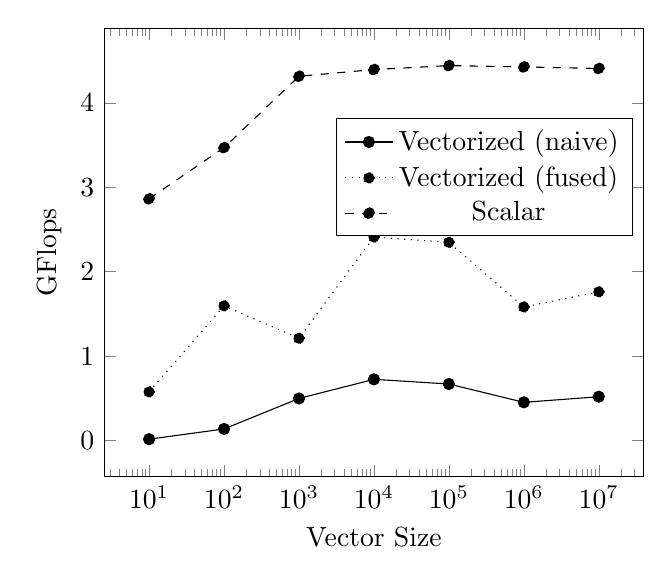
\begin{tikzpicture}
\begin{semilogxaxis}[
    %title=Vectorization Performance,
    xlabel={Vector Size},
    ylabel={GFlops},
    legend entries={Vectorized (naive), Vectorized (fused), Scalar},
    legend style={at={(0.98,0.8)}},
]
\addplot+[color=black,mark=*,mark options={fill=black}] coordinates {
%(10, 0.0192)
%(100, 0.1547)
%(1000, 0.4921)
%(10000, 0.6890)
%(100000, 0.5958)
%(1000000, 0.5380)
%(10000000, 0.3741)
(10, 0.0181)
(100, 0.1390)
(1000, 0.5001)
(10000, 0.7263)
(100000, 0.6714)
(1000000, 0.4543)
(10000000, 0.5208)

};
\addplot+[color=black,mark=*,mark options={fill=black},style=dotted] coordinates {
%(10, 0.5970)
%(100, 1.9327)
%(1000, 1.1569)
%(10000, 2.1719)
%(100000, 2.1416)
%(1000000, 1.4537)
%(10000000, 1.2961)
(10, 0.5778)
(100, 1.5960)
(1000, 1.2126)
(10000, 2.4110)
(100000, 2.3484)
(1000000, 1.5835)
(10000000, 1.7621)

};
\addplot+[color=black,mark=*,mark options={fill=black},style=dashed] coordinates {
%(10, 2.6954)
%(100, 3.4087)
%(1000, 4.2119)
%(10000, 4.3665)
%(100000, 4.3804)
%(1000000, 4.3789)
%(10000000, 4.4510)
(10, 2.8637)
(100, 3.4693)
(1000, 4.3138)
(10000, 4.3934)
(100000, 4.4404)
(1000000, 4.4245)
(10000000, 4.4061)

};
\end{semilogxaxis}
\end{tikzpicture}
\caption{
  Performance of evaluating $x^2+x+1$ over a vector.
}
\label{vecperf}
\end{figure}

\subsection{Vandermonde matrix case study}

\begin{singlespace}
\begin{lstlisting}[language=python,style=ttcode]
def vander(x, N):
  x = asarray(x)
  if x.ndim != 1:
    raise ValueError("x must be a one-dimensional array or sequence.")

  v = empty((len(x), N), dtype=promote_types(x.dtype, int))

  if N > 0:
    v[:, 0] = 1
  if N > 1:
    v[:, 1:] = x[:, None]
    multiply.accumulate(v[:, 1:], out=v[:, 1:], axis=1)

  return v
\end{lstlisting}
\end{singlespace}


\begin{singlespace}
\begin{lstlisting}[language=julia]
function vander{T}(x::Array{T,1}, N::Int)
  m = length(x)
  V = Array(T, m, N)
  if N > 0
    V[:, 1] = 1
  end
  for i = 2:N
    for j = 1:m
      V[j,i] = x[j] * V[j,i-1]
    end
  end
  return V
end
\end{lstlisting}
\end{singlespace}

\subsection{What needs to be built in?}

On``built-in", why built-in is bad.

Built-in-ness often conflates two aspects:

\begin{enumerate}
\item A feature being readily available and agreed-on by all language users
\item A feature tightly coupled to the rest of the system
\end{enumerate}

(2) implies (1), but not the other way around. (2) is the only technically
interesting item, since the other can be addressed e.g.\  just by including
a library in the standard software distribution. Many technical computing
languages have done a large amount of (2) while justifying it with point (1).


While a large part of our motivation is to move more decisions and functionality
into libraries, it is equally important to identify what {\it  must} be part of a
language for the system to be successful. We believe that large amounts of
functionality can be provided by add-ons, but that certain key features
cannot be. Past failures to properly classify features this way have
caused a lot of undue pain.

First, performance cannot be an add-on. If some users have a fast version of
a language and others have a slow version (with the difference being an
order of magnitude or more), library writers cannot be sure whether users
will find their code fast enough to be useful. How are we to teach people to
program in the language? Courses on MATLAB programming emphasize vectorized code,
but if not all implementations had this performance characteristic,
presumably curricula would need to change.\todo{Comment, I do not think they all do and curricula therefore must change}

Psychologically, it may be difficult to accept a ``non standard'' extension
that changes a language so fundamentally. There is a nagging, though perhaps
totally unfounded, perception that something subtle may break. If indeed a
bug arises due to the use of such an extension, a user is likely to conclude
that the extension is dangerous or broken and stop using it. If, on the other
hand, a bug arises due to a language's standard optimizing compiler, the user
will simply file a bug report, then find a way to work around the problem.

Adding a JIT compiler to a language also requires acceptance of detriments
like compilation pauses and pages with RWX permissions. In some cases this
may lead to use of the extension being disallowed, perhaps for security
reasons.

Type systems similarly fail when provided as optional extensions. Library
writers face the same kinds of problems as with performance add-ons. Should I
use type annotations in my library?

Dynamic dispatch mechanisms also make especially poor add-ons. Of course,
every program makes decisions at run time, and so implements its own
``dispatch'' to some extent. But these behaviors are inextensible; if
language users do not agree on a reusable dispatch framework their code
will not be composable.


\section{Social phenomena}

Programming languages are observed to have strong network effects, and the
difficulty of getting new languages adopted is well known. However based on
\cite{meyerovich2012socio} we believe this doesn't have to be the case.
The formula
of improving or redesigning general-purposes languages to be more appealing to
domain experts might solve the problem. That way the new system has immediate
appeal for at least some users, without the worry that a different tool will
be needed as soon as requirements change slightly.

Barriers to contributing.

%Debates about what abstractions mean -- AbstractMatrix
%we thought we knew what it meant, but what about something like
%SymTridiagonal? It can implement most of what a dense matrix
%has, but it can't obey every invariant.

%PackedQR
